\subsubsection{bringit::client::view:item::inputitem::InputItemInfoView}

\label{bringit::client::view:item::inputitem::InputItemInfoView}
\begin{figure}[H]
	\centering
	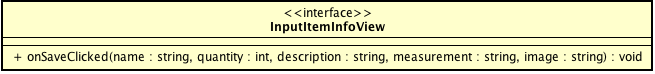
\includegraphics[scale=0.5]{Sezioni/SottosezioniST/img/app/InputItemInfoView.png}
	\caption{bringit::client::view:item::inputitem::InputItemInfoView}
\end{figure}

\begin{itemize}
\item \textbf{Descrizione}: La view relativa all'input delle informazioni degli oggetti da aggiungere a una lista.
\item \textbf{Utilizzo}: L'interfaccia viene utilizzata per disaccoppiare presenter e implementazione della classe e per visualizzare i dati che gli vengono passati dal presenter.
\item \textbf{Attributi}: 
\item \textbf{Metodi}:
	\begin{itemize}
	\item \textit{public onSaveClicked(name:string,quantity:string,description:string,measurement:string,image:blob):void}\\
	Questo metodo chiama la funzione per la creazione dell'item della lista utilizzando i parametri inseriti.
				\\ \textbf{Parametri}: \begin{itemize}
			\item \textit{name:string}\\
			Il nome del prodotto.
			\item \textit{quantity:string}\\
			La quantità relativa al prodotto.
			\item \textit{description:string}\\
			La descrizione del prodotto.
			\item \textit{measurement:string}\\
			L'unità di misura per il prodotto in questione.
			\item \textit{image:blob}\\
			L'immagine del prodotto.
					\end{itemize} 
	\end{itemize}
\end{itemize} 

\subsubsection{bringit::client::view:item::inputitem::view::InputItemInfoViewImpl}

\label{bringit::client::view:item::inputitem::view::InputItemInfoViewImpl}
\begin{figure}[H]
	\centering
	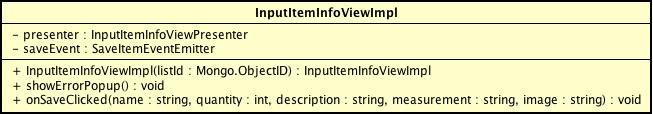
\includegraphics[scale=0.5]{Sezioni/SottosezioniST/img/app/InputItemInfoViewImpl.png}
	\caption{bringit::client::view:item::inputitem::view::InputItemInfoViewImpl}
\end{figure}

\begin{itemize}
\item \textbf{Descrizione}: Questa classe rappresenta il form di inserimento delle informazioni di un item della lista, implementando l'interfaccia.
\item \textbf{Utilizzo}: Implementando i metodi di InputItemInfoView questa classe viene utilizzata al momento dell'inserimento delle informazioni relative ad un item della lista bringit.
\item \textbf{Attributi}: 
	\begin{itemize}
	\item \textit{private listId:string}\\
	L'identificativo della lista alla quale si sta aggiungendo l'item.
	\item \textit{private presenter:InputItemViewPresenter}\\
	Il presenter relativo all'input delle informazioni di un prodotto della lista.
	\end{itemize}
\item \textbf{Metodi}:
	\begin{itemize}
	\item \textit{public InputItemInfoViewImpl(listId:string):InputItemInfoViewImpl}\\
	Il costruttore della classe InputItemInfoViewImpl.
					\\ \textbf{Parametri}: \begin{itemize}
			\item \textit{listId:string}\\
			L'identificativo della lista alla quale si sta aggiungendo l'item
					\end{itemize} 
	\item \textit{public onSaveClicked(name:string,quantity:string,description:string,measurement:string,image:blob):void}\\
	Questo metodo chiama la funzione per la creazione dell'item della lista utilizzando i parametri inseriti.
				\\ \textbf{Parametri}: \begin{itemize}
			\item \textit{name:string}\\
			Il nome del prodotto.
			\item \textit{quantity:string}\\
			La quantità relativa al prodotto.
			\item \textit{description:string}\\
			La descrizione del prodotto.
			\item \textit{measurement:string}\\
			L'unità di misura per il prodotto in questione.
			\item \textit{image:blob}\\
			L'immagine del prodotto.
					\end{itemize} 
		\item \textit{public showErrorPopup():void}\\
		Questo metodo mostra un popup di errore nel caso si tenti di inserire un prodotto senza nome.	
	\end{itemize}
\end{itemize}

\subsubsection{bringit::client::view:item::inputitem::presenter::InputItemInfoViewPresenter}

\label{bringit::client::view:item::inputitem::presenter::InputItemInfoViewPresenter}
\begin{figure}[H]
	\centering
	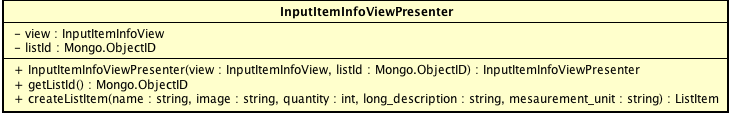
\includegraphics[scale=0.5]{Sezioni/SottosezioniST/img/app/InputItemInfoViewPresenter.png}
	\caption{bringit::client::view:item::inputitem::presenter::InputItemInfoViewPresenter}
\end{figure}

\begin{itemize}
\item \textbf{Descrizione}: Questa classe rappresenta il presenter per la classe di inserimento dei dati di un item della lista.
\item \textbf{Utilizzo}: Il presenter fa da tramite tra l'implementazione e la view, formattando i dati che verranno visualizzati nella view e manipolando gli input dell'utente per eseguire le operazioni logiche predisposte.
\item \textbf{Attributi}: 
	\begin{itemize}
	\item \textit{private listId:string}\\
	L'identificativo della lista alla quale si sta aggiungendo l'item
	\item \textit{private view:InputItemInfoView}\\
	La view necessaria alla costruzione del presenter.
	\end{itemize}
\item \textbf{Metodi}:
	\begin{itemize}
	\item \textit{public InputItemInfoViewPresenter(listId:string,view:InputItemInfoView):InputItemInfoViewPresenter}\\
	Il costruttore della classe InputItemInfoViewPresenter.
					\\ \textbf{Parametri}: \begin{itemize}
			\item \textit{listId:string}\\
			L'identificativo della lista alla quale si sta aggiungendo l'item
			\item \textit{view:InputItemInfoView}\\
			La view necessaria alla costruzione del presenter.
					\end{itemize} 
	\item \textit{public showErrorPopup():void}\\
	Questo metodo crea l'oggetto della lista con i parametri specificati e ritorna la lista alla quale lo si sta aggiungendo.
	\item \textit{public createListItem(name:string, image:blob, quantity:string, long\_description:string, mesaurement\_unit:string):ListData}
						\\ \textbf{Parametri}: \begin{itemize}
			\item \textit{name:string}\\
			Il nome del prodotto.
			\item \textit{image:blob}\\
			L'immagine del prodotto.
			\item \textit{quantity:string}\\
			La quantità relativa al prodotto.
			\item \textit{long\_description:string}\\
			La descrizione del prodotto.
			\item \textit{mesaurement\_unit:string}\\
			L'unità di misura relativa al prodotto.
					\end{itemize}
	\end{itemize}
\end{itemize}

\subsubsection{bringit::client::view:item::showinfoitem::ShowInfoItem}

\label{bringit::client::view:item::showinfoitem::ShowInfoItem}
\begin{figure}[H]
	\centering
	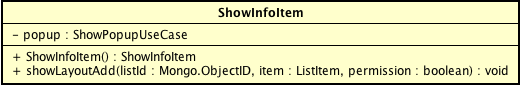
\includegraphics[scale=0.5]{Sezioni/SottosezioniST/img/app/ShowInfoItem.png}
	\caption{bringit::client::view:item::showinfoitem::ShowInfoItem}
\end{figure}

\begin{itemize}
\item \textbf{Descrizione}: Questa classe rappresenta il modale per la visualizzazione dei dettagli aggiuntivi di un item di una lista bringit.
\item \textbf{Utilizzo}: La classe viene utilizzata per comunicare agli utenti i dettagli di un oggetto della lsita bringit. Inoltre tramite questo popup si può modificare o rimuovere l'item in questione
\item \textbf{Attributi}: 
	\begin{itemize}
	\item \textit{private popup:ShowPopupUseCase}\\
	La classe necessaria alla gestione dei popup in bringit.
	\end{itemize}
\item \textbf{Metodi}:
	\begin{itemize}
	\item \textit{public ShowInfoItem():ShowInfoItem}\\
	Il costruttore della classe ShowInfoItem.
		\item \textit{public showLayoutAdd(listId:string,item:ItemList,permission:boolean):void}\\
		Questo metodo mostra un popup con le informazioni aggiuntive di un item di una lista bringit.
					\\ \textbf{Parametri}: \begin{itemize}
			\item \textit{listId:string}\\
			L'identificativo della lista della quale si vuole mostrare le informazioni aggiuntive di un item.
			\item \textit{item:ItemList}\\
			L'item del quale si vogliono mostrare le informazioni aggiuntive.
			\item \textit{permission:boolean}\\
			Il booleano che rappresenta i permessi, e che se impostato a true rende possibile la modifica o la rimozione dell'item in questione.
					\end{itemize} 
	\end{itemize}
\end{itemize}